\documentclass[a4paper, 11pt]{article}
\usepackage{fullpage}
\usepackage{mathtools, nccmath}
\usepackage{graphicx}
\usepackage{float}
\usepackage{amsmath}
\renewcommand{\figurename}{Fig.}
\renewcommand{\refname}{Bibliografia}

\begin{document}
% Header
\noindent
\large\textbf{Corso di Metodi di Ottimizzazione} \hfill \textbf{Gruppo E} \\
\normalsize A.A. 2018/2019 \hfill Ing. Saverio Del Prete \\
Prof. Raffaele Martone \hfill Ing. Bernardo Giordano \\
\hphantom{}\hfill Ing. Lucia Migliaccio

\section*{Traccia del problema}

Progetto ottimo di un campo magnetico con incognite geometriche e di corrente di
una spira.

\section*{Descrizione del sistema fisico}

Il sistema è composto da un certo numero di spire simmetriche (supporremo $n=6$)
concentriche rispetto allo stesso asse $z$. I parametri di progetto, ovvero
posizione, raggio e intensità di corrente, sono noti per tutte le spire tranne
che per una coppia.

\begin{figure}[H]
	\centering
	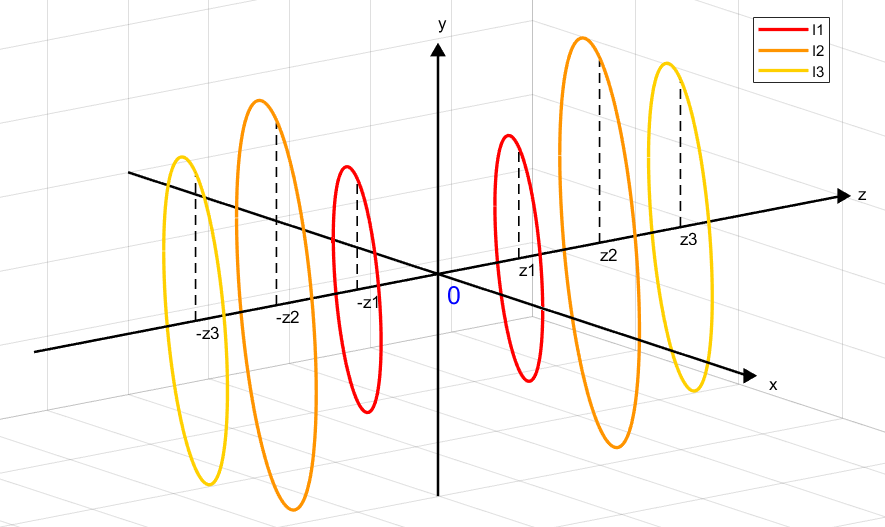
\includegraphics[width=12cm]{assets/figure1}
	\caption{Schematizzazione del sistema fisico.}
\end{figure}
\noindent

Il campo magnetico generato dalla corrente circolante nelle spire può essere
valutato sull’asse utilizzando la legge di Biot-Savart. La legge di Biot-Savart
permette di valutare il campo magnetico B prodotto in un punto dello spazio da
una spira percorsa da corrente elettrica. \\ \\
\noindent
Il campo magnetico sull’asse $z$  di una spira caratterizzata da una corrente
$I$, lunghezza $L$, raggio $R$ e posizione $Z$ si valuta come
\[dB_{z}=\frac{\mu_{0}IdL}{4\pi}\frac{R}{\left((Z{\pm}z)^{2}+R^{2}\right)^{3/2}}\]
dove $\mu_{0}$ è la permeabilità magnetica nel vuoto, $\mu_{0}=4{\pi}10^{-7}
H/m$. \\
L’integrale di $dL$ risulta essere proprio la circonferenza della spira, ovvero
$2{\pi}R$. Integrando quindi, si ricava la funzione del campo magnetico
sull'asse
\[B_{z}=\frac{\mu_{0}}{4\pi}\frac{2{\pi}R^{2}I}{\left((Z{\pm}z)^{2}+R^{2}\right)^{3/2}}=\frac{\mu_{0}}{2}\frac{R^{2}I}{\left((Z{\pm}z)^{2}+R^{2}\right)^{3/2}}\]
Siano $Z_{i}$, $R_{i}$ e $I_{i}$ rispettivamente la posizione, il raggio e la
corrente relative alla spira $i$-esima. \\
Sia inoltre $n=6$ il numero complessivo delle spire facenti parte del sistema.
Considerando adesso la sovrapposizione degli effetti di tutte le spire del
sistema e tenendo presente che le spire sono simmetriche rispetto al piano
$r{\theta}$, il campo magnetico complessivo sull’asse $z$ sarà:

\begin{align*}
	B_{z}
	&=\frac{\mu_{0}}{4{\pi}}\left(\sum_{i=1}^{n/2}\frac{2{\pi}I_{i}R_{i}^{2}}{\left(\left(Z_{i}-z\right)^{2}+R_{i}^{2}\right)^{3/2}}+\frac{2{\pi}I_{i}R_{i}^{2}}{\left(\left(Z_{i}+z\right)^{2}+R_{i}^{2}\right)^{3/2}}\right)\\
	&=\frac{\mu_{0}}{2}\left(\sum_{i=1}^{n/2}\frac{I_{i}R_{i}^{2}}{\left(\left(Z_{i}-z\right)^{2}+R_{i}^{2}\right)^{3/2}}+\frac{I_{i}R_{i}^{2}}{\left(\left(Z_{i}+z\right)^{2}+R_{i}^{2}\right)^{3/2}}\right)
\end{align*}
\noindent

L'obiettivo del progetto della spira mancante risulta essere la migliore
approssimazione di un campo magnetico avente la seguente caratteristica:

\begin{figure}[H]
	\centering
	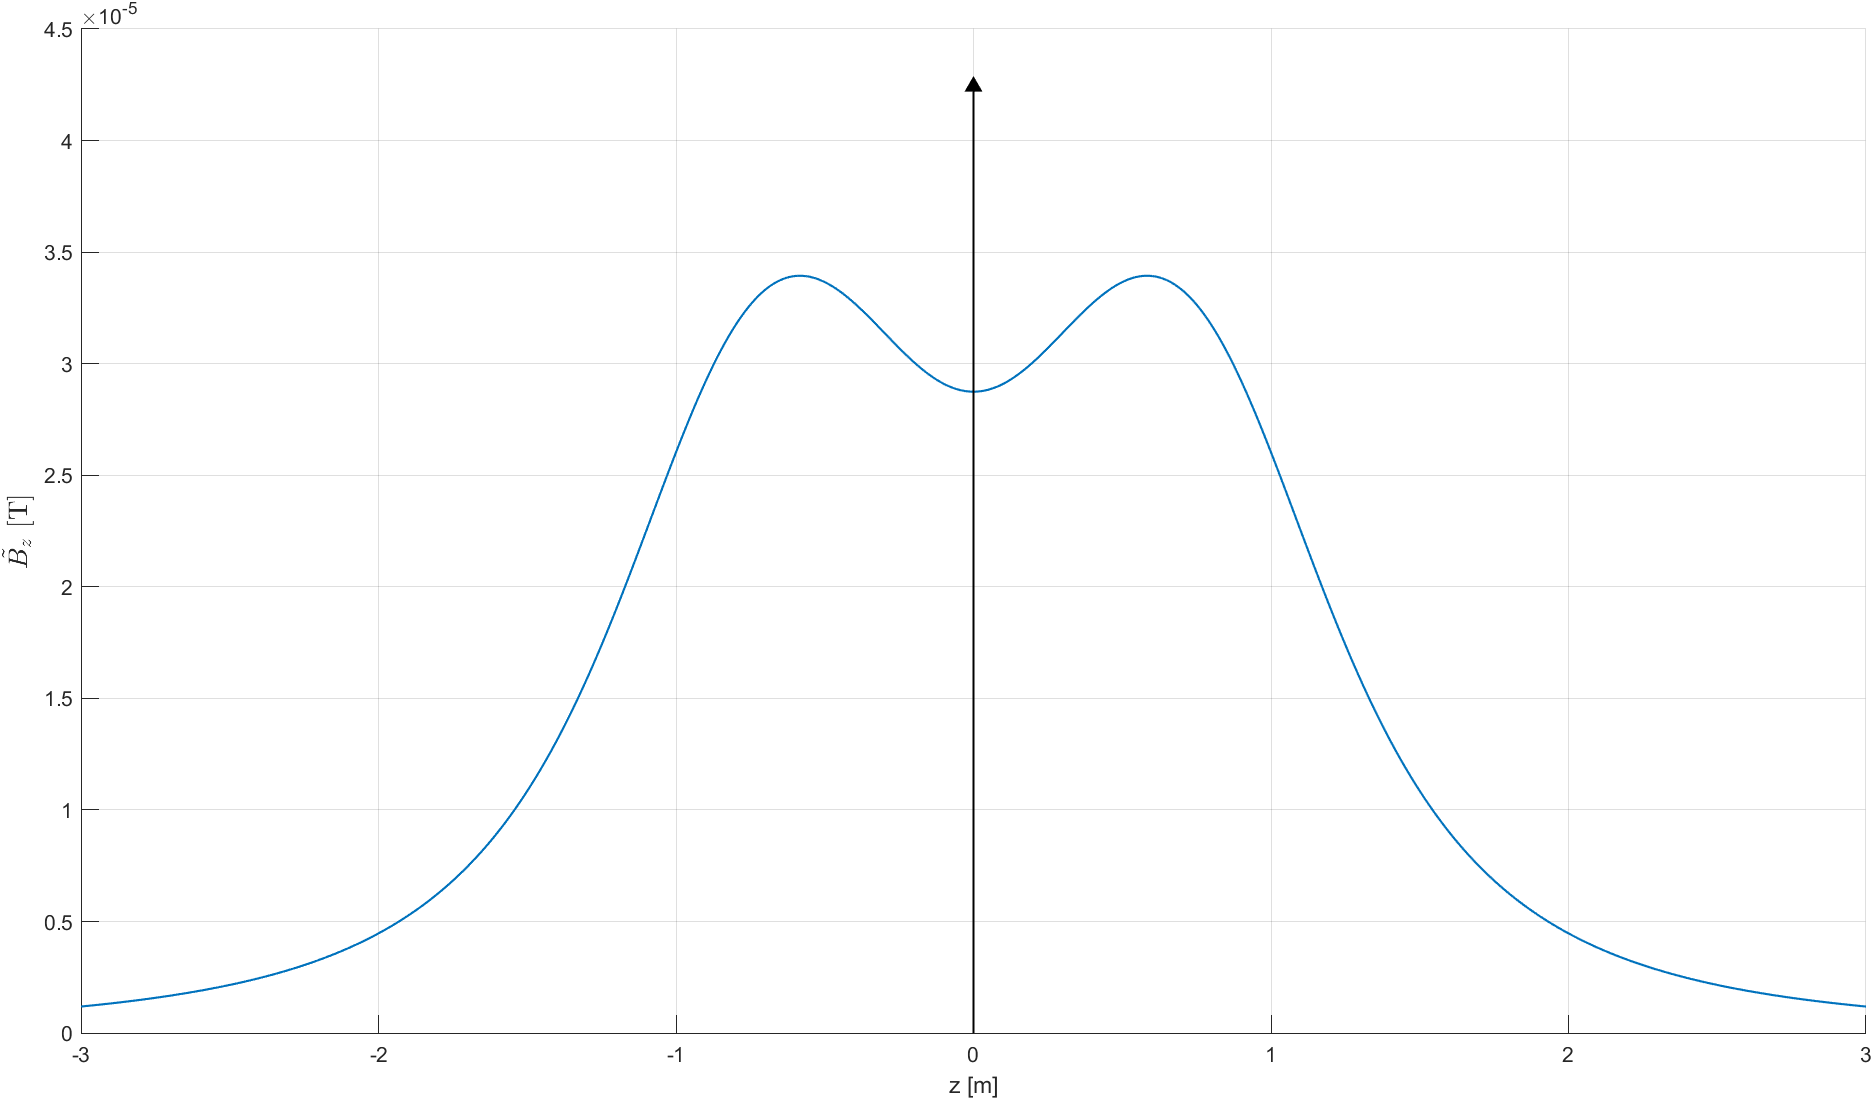
\includegraphics[width=16cm]{assets/figure2}
	\caption{Campo magnetico sull'asse $z$ desiderato.}
\end{figure}
\noindent
Sia adesso $B_{z}$ il campo magnetico generato dalla sovrapposizione delle spire
del sistema, e $\tilde{B_{z}}$ il campo magnetico desiderato. Al fine da
ottenere una discrepanza più piccola possibile, è di particolare interesse lo
studio del minimo della funzione
\[||B_{z}-\tilde{B_{z}}||\] Siccome i parametri di progetto delle spire 1 e 3
del sistema (e, quindi, delle rispettive spire simmetriche) sono noti ed
esattamente uguali a quelli del sistema desiderato, la suddetta differenza in
norma si scriverà come:

\begin{equation}
	\begin{split}
		||B_{z}-\tilde{B_{z}}||
		=& \Bigl|\Bigl|\frac{\mu_{0}}{2}(\frac{I_{2}R_{2}^{2}}{((Z_{2}-z)^{2}+R_{2}^{2})^{3/2}}+\frac{I_{2}R_{2}^{2}}{((Z_{2}+z)^{2}+R_{2}^{2})^{3/2}})+ \\
		 & -\frac{\mu_{0}}{2}(\frac{\tilde{I_{2}}\tilde{R_{2}}^{2}}{((\tilde{Z_{2}}-z)^{2}+\tilde{R_{2}}^{2})^{3/2}}-\frac{\tilde{I_{2}}\tilde{R_{2}}^{2}}{((\tilde{Z_{2}}+z)^{2}+\tilde{R_{2}}^{2})^{3/2}})\Bigr|\Bigr| \\
		=& \frac{\mu_{0}}{2}\Bigl|\Bigl|\frac{I_{2}R_{2}^{2}}{((Z_{2}-z)^{2}+R_{2}^{2})^{3/2}}+\frac{I_{2}R_{2}^{2}}{((Z_{2}+z)^{2}+R_{2}^{2})^{3/2}}+ \\
		 & -\frac{\tilde{I_{2}}\tilde{R_{2}}^{2}}{((\tilde{Z_{2}}-z)^{2}+\tilde{R_{2}}^{2})^{3/2}}-\frac{\tilde{I_{2}}\tilde{R_{2}}^{2}}{((\tilde{Z_{2}}+z)^{2}+\tilde{R_{2}}^{2})^{3/2}}\Bigr|\Bigr|
	\end{split} 
\end{equation}
\noindent

\section*{Campionamento e normalizzazione}

Prima di poter definire la funzione obiettivo ed effettuarne un'analisi
numerica, è necessario applicare due tecniche: campionamento e normalizzazione.
\\
Il campionamento è una tecnica che consiste nel discretizzare una funzione
continua nel tempo. L'ampiezza del passo di campionamento può essere valutato a
intervalli temporali regolari e non. \\
In questo caso specifico, si è deciso di utilizzare un campionamento a passo
costante. \\
La normalizzazione è l'operazione la quale, dato un vettore, lo si porta ad
avere una norma unitaria. \\
% aggiungere altre cose sulla normalizzazione
La funzione verrà campionata su $N_{p}$ valori dell'asse $z$. La funzione
campionata, inoltre, verrà normalizzata e mediata sul valor medio di
$\tilde{B_{z}}$, in modo tale da esprimere la funzione obiettivo come
percentuale di scostamento tra il campo magnetico progettato e quello ideale. \\
Campionando e normalizzando la (1), la \emph{funzione obiettivo} si scriverà
come:
 
\begin{equation}
	\begin{split}
		F_{obj}(I_{2},R_{2},Z_{2}) =
		& \frac{1}{{\tiny <} \tilde{B_{z}}{\tiny >}} \Biggl[ \frac{1}{Np} \sum\limits_{k=1}^{Np} \Bigl|\Bigl|\frac{I_{2}R_{2}^{2}}{((Z_{2}-z_{k})^{2}+R_{2}^{2})^{3/2}}+\frac{I_{2}R_{2}^{2}}{((Z_{2}+z_{k})^{2}+R_{2}^{2})^{3/2}}+ \\
		& -\frac{\tilde{I_{2}}\tilde{R_{2}}^{2}}{((\tilde{Z_{2}}-z_{k})^{2}+\tilde{R_{2}}^{2})^{3/2}}-\frac{\tilde{I_{2}}\tilde{R_{2}}^{2}}{((\tilde{Z_{2}}+z_{k})^{2}+\tilde{R_{2}}^{2})^{3/2}}\Bigr|\Bigr|^{2}\biggr]^{\!1/2}
	\end{split} 
\end{equation}
\noindent

\section* {Ricerca del minimo}

L'algoritmo di ricerca del minimo fa uso del concetto di simplesso, cioè un
politopo di $N+1$ vertici in $N$ dimensioni, vale a dire: un segmento in una
dimensione, un triangolo in due dimensioni, un tetraedro in tre dimensioni, e
così via. Il metodo permette di limitare la ricerca della soluzione ottima ai
vertici del politopo. \\
La ricerca avviene attraverso il movimento del politopo, il quale può:

\begin{itemize}
\item \textbf{Ribaltarsi}: si valuta la funzione negli $N$ vertici del
simplesso, individuando qual è il vertice nel quale la funzione assume il valore
\emph{peggiore} (nel caso di un problema di ricerca del minimo, il caso peggiore
è quello in cui la funzione assume valore più grande tra tutti i vertici del
simplesso considerato). Una volta identificato il vertice peggiore, il simplesso
si ribalta rispetto a quest'ultimo, tenendo fermi gli altri $N-1$ vertici. \\
L'algoritmo può però ritrovarsi in una situazione di loop, dove il vertice
peggiore risulta essere proprio l'ultimo rispetto al quale è stato effettuato il
ribaltamento. In questo caso, si ribalta rispetto al \emph{secondo peggior
vertice}. 
\item \textbf{Contrarsi}: se un vertice del politopo \emph{vive} più a lungo di
un numero arbitrario di iterazioni $M$, il politopo viene contratto, dimezzando
i lati dell'ultimo simplesso tenendo fermo il vertice \emph{migliore}.
\end{itemize}

\noindent
L'algoritmo di ricerca del minimo mediante l'uso del politopo è un metodo di
\emph{ordine 0}, ovvero non richiede l'uso delle derivate, nonostante riesca a
stimare una direzione di discesa della funzione obiettivo.

\section*{Implementazione dell'algoritmo}

L'algoritmo implementato per la soluzione del problema della ricerca del minimo
consiste in una fase di \emph{inizializzazione}, una di \emph{loop} (nella quale
vengono effettuate tutte le operazioni di ribaltamento e contrazione del
simplesso) e una di \emph{controllo delle condizioni di arresto} del loop. \\ \\
La fase di inizializzazione consiste nell'impostazione di tutte le variabili
necessarie al funzionamento dell'algoritmo, che per design vengono
parametrizzate, in modo tale da rendere comodo l'utilizzo dell'algoritmo in
differenti condizioni iniziali, tra cui:
\begin{itemize}
\item \textbf{Passo di campionamento}, necessario all'approssimazione più o meno
grossolana della funzione obiettivo da studiare.
\item \textbf{Range dei parametri liberi}, con i quali si stabiliscono due
valori limite che dovranno essere rispettati da tutte le variabili da
ottimizzare.
\item \textbf{Condizioni di arresto}, necessarie per stabilire fino a quanto
l'algoritmo dovrà iterare per garantire dei risultati soddisfacenti. Tra le
innumerevoli condizioni possibili, verranno considerate il \emph{massimo numero
di ribaltamenti}, un valore di \emph{massimo errore percentuale} rispetto alla
funzione desiderata e un vincolo sulla \emph{minima lunghezza del lato} del
simplesso generato ad ogni passi.
\item \textbf{Punto iniziale}, che condizionerà, insieme all'andamento della
funzione, la generazione di determinati simplessi piuttosto che altri.
\end{itemize}

\noindent
Una volta parametrizzate le condizioni iniziali, l'algoritmo entrerà in fase di
loop, dove eseguirà ripetutamente le seguenti operazioni:

\begin{enumerate}
\item Un simplesso iniziale $s$ con centroide in $s_{0}$ viene aggiunto ad un
array di simplessi $polytope$
\item Controllo se un vertice di $s = polytope(end)$ ha vissuto per $k$
iterazioni
\item Se si:
\begin{enumerate}
\item Trovo il vertice $i$ di $s$ dove $F_{obj}$ assume valore minore
\item Dimezzo la lunghezza dei lati di $s$ lasciando fermo il vertice $i$,
ottenendo $s_{new}$
\end{enumerate}
\item Se no:
\begin{enumerate}
\item Trovo il vertice $i$ di $s$ dove $F_{obj}$ assume valore massimo
\item Ribalto $s$ tenendo fermi i vertici $k \ne i$, ottenendo $s_{new}$
\item Se $F_{obj}(s(i)) \leq F_{obj}(s_{new}(i))$:
\begin{enumerate}
\item Trovo il secondo vertice $j$ di $s$ dove $F_{obj}$ assume valore massimo
\item Ribalto $s$ tenendo fermi i vertici $k \ne j$, ottenendo $s_{new}$
\end{enumerate}
\end{enumerate}
\item Aggiungo $s_{new}$ a $polytope$, $polytope(end+1) = s_{new}$
\item Interrompi se almeno una condizione di arresto è verificata, altrimenti
ripeti dal passo 2.
\end{enumerate}

\noindent
L'algoritmo può essere schematizzato in maniera compatta secondo il seguente
diagramma di flusso:

% INSERIRE DIAGRAMMA

\section*{Scelta dei parametri}

Al fine di avvicinarci alla caratteristica descritta in $Fig. 2$, vanno scelti
opportunamente il valore dei raggi, delle correnti e delle posizioni relative a
tutte le spire, comprese quelle da progettare (spire 2 e 4). \\ \\
\centerline{ \textbf{Spira 1}: $R_{1}$ = 0.7m \\ $I_{1}$ = 3 A \\ $Z_{1}$ = -0.4m} 
\centerline{ \textbf{Spira 2}: $R_{2}$ = 0.8m \\ $I_{2}$ = 5 A \\ $Z_{2}$ = -0.7m}
\centerline{ \textbf{Spira 3}: $R_{3}$ = 0.6m \\ $I_{3}$ = 2 A \\ $Z_{3}$ = -0.9m}
\centerline{ \textbf{Spira 4}: $R_{4}$ = 0.7m \\ $I_{4}$ = 3 A \\ $Z_{4}$ = 0.4m}
\centerline{ \textbf{Spira 5}: $R_{5}$ = 0.8m \\ $I_{5}$ = 5 A \\ $Z_{5}$ = 0.7m}
\centerline{ \textbf{Spira 6}: $R_{6}$ = 0.6m \\ $I_{6}$ = 2 A \\ $Z_{6}$ = 0.9m}

\section*{Esperimenti}


\begin{thebibliography}{9}
	% \bibitem{id}Author\emph{title}[online]. Editor.
\end{thebibliography}
\end{document}